\documentclass[12pt,onecolumn,notitlepage]{article}
\usepackage[margin=0.5in]{geometry}
\usepackage{amsmath}
\usepackage{gensymb}
\usepackage{graphicx}
\usepackage{amsthm}
\usepackage{mathrsfs}
\usepackage{txfonts}
\usepackage{cite}
\usepackage{cases}
\usepackage{subfig}
\usepackage[breaklinks=true]{hyperref}
\usepackage{listings}
\usepackage[latin1]{inputenc}
\usepackage{color}
\usepackage{array}
\usepackage{longtable}
\usepackage{calc}
\usepackage{multirow}
\usepackage{hhline}
\usepackage{ifthen}
\usepackage{amssymb}
\usepackage{hyperref}

\providecommand{\pr}[1]{\ensuremath{\Pr\left(#1\right)}}
\providecommand{\sbrak}[1]{\ensuremath{{}\left[#1\right]}}
\providecommand{\lsbrak}[1]{\ensuremath{{}\left[#1\right.}}
\providecommand{\rsbrak}[1]{\ensuremath{{}\left.#1\right]}}
\providecommand{\brak}[1]{\ensuremath{\left(#1\right)}}
\providecommand{\lbrak}[1]{\ensuremath{\left(#1\right.}}
\providecommand{\rbrak}[1]{\ensuremath{\left.#1\right)}}
\providecommand{\cbrak}[1]{\ensuremath{\left\{#1\right\}}}
\providecommand{\lcbrak}[1]{\ensuremath{\left\{#1\right.}}
\providecommand{\rcbrak}[1]{\ensuremath{\left.#1\right\}}}
\newcommand*{\comb}[2]{{}^{#1}C_{#2}}
\title{Software Assignment Report}
\author{Pallala Rishitha (BT22BTECH11011)}
\date{}
\begin{document}
\maketitle
\textbf{\LARGE{Assignment :}}\\\\Code is written to take to take audio playlist and shuffle them using random variables. User interface has been created which has the options to 'shuffle and play' and 'Exit' from the user interface.\\\\
\textbf{\LARGE{Analysis of code:}}

   \section*{Libraries imported :}
\begin{enumerate}
  \setlength\itemsep{0pt} % Adjust the spacing between points
  \item     tkinter is used for creating the graphical user interface.
    \item numpy is used for shuffling the playlist.
    \item pygame is used for audio playback.
\end{enumerate} 
   \section*{Defining the 'AudioPlaylistUI' class::}
\begin{enumerate}
  \setlength\itemsep{0pt}
  \item AudioPlaylistUI class is responsible for creating and managing the user interface.
  \item init method is the class constructor and sets up the initial state of the interface.
\end{enumerate} 
 
\section*{Initializing the interface:}
\begin{enumerate}
  \setlength\itemsep{0pt}
      \item  tk.Listbox widget is used to display and manage the playlist of audio files.
    \item  widget is packed into the interface window with a vertical padding of 10 pixels.
\end{enumerate} 
 
 
\section*{Adding the "Shuffle and Play" button:}
\begin{enumerate}
  \setlength\itemsep{0pt}
     \item tkButton widget is created with the text Shuffle and Play and assigned the command selfshuffleandplay .
    \item When the button is clicked, it will call the shuffleandplay method of the class.
    \item  button is packed into the interface window with a vertical padding of 5 pixels.


\end{enumerate} 
 
 
\section*{Adding the "Exit" button:}
\begin{enumerate}
  \setlength\itemsep{0pt}
  \item     The tkButton widget is created with the text "Exit" and assigned the command selfexit interface.
   \item When the button is clicked, it will call the exit interface method of the class.
    \item The button is packed into the interface window with a vertical padding of 5 pixels.
\end{enumerate} 
\section*{Defining the shuffle and play method:}
\begin{enumerate}
  \setlength\itemsep{0pt}
  \item     The shuffle and play method is called when the "Shuffle and Play" button is clicked.
   \item It shuffles the items in the playlist by converting them to a list, shuffling the list, and updating the playlist accordingly.
   \item The playlist index is set to 0 to start playing from the beginning.
   \item The playing flag is set to True to indicate that the playlist is being played.
    \item The play next method is called to start playing the shuffled playlist.
\end{enumerate} 
 \section*{Defining the play next method:}
\begin{enumerate}
  \setlength\itemsep{0pt}
  \item     The play next method is responsible for playing the next audio file in the shuffled playlist.
    \item It checks if the playback is still ongoing (selfplaying) and if there are more items in the playlist to play.
    \item It gets the audio file path from the current playlist index, loads the file into pygamemixermusic, and plays it.
    \item It waits for the playback to finish using a while loop and then increments the playlist index to move to the next item.
    \item It calls itself recursively to play the next audio file until the end of the playlist is reached.
    \item When the playlist is finished, the playing flag is set to False.


\end{enumerate} 
 \section*{Defining the exit interface method:}
\begin{enumerate}
  \setlength\itemsep{0pt}
  \item     The exit interface method is called when the "Exit" button is clicked.
   \item  It stops the current playback by setting the playing flag to False and stopping the music using pygamemixermusicstop().
    \item It destroys the interface window by calling selfmasterdestroy().
\end{enumerate} 
\section*{Creating the interface window and running the event loop:}
\begin{enumerate}
  \setlength\itemsep{0pt}
  \item     The tkTk() function creates the main window for the interface.
   \item  An instance of the AudioPlaylistUI class is created with the window as the master parameter.
    \item The rootmainloop() call starts the event loop, which listens for user interactions and updates the interface accordingly.
\end{enumerate} 
\textbf{\LARGE{How the code works:}}\\
 \large{By running this code, you will have a graphical user interface with the "Shuffle and Play" and "Exit" buttons Clicking the "Shuffle and Play" button will shuffle the playlist and start playing the audio files. Clicking the "Exit" button will stop the playback and close the interface window.}\\
 
 
 \begin{figure}[h!]
  \centering
  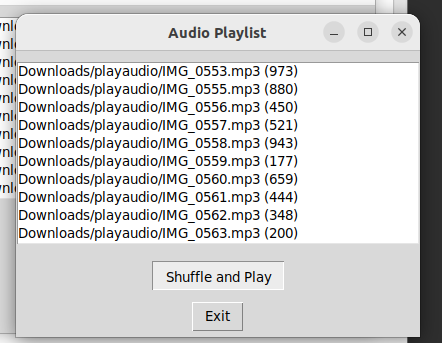
\includegraphics[width=0.5\textwidth]{playlistui.png}
  \caption{User Interface for the Playlist }
  \label{fig:graphical user interface}
\end{figure}
\textbf{\large{codes:}}\\
\href{https://github.com/rishithapallala/AI1110/blob/main/software_assignment/playlist.py}{click here for Github link of the python code of the playlist}


\end{document}
